\subsection{Slučaj upotrebe: Prijava na sistem}

\subsubsection*{Kratak opis}

Zaposleni se prijavljuje na sistem unosom korisničkog imena i lozinke, kako bi dobio pristup funkcionalnostima u skladu sa svojom ulogom.

\subsubsection*{Akteri}
\begin{itemize}
	\item \textbf{Zaposleni} -- svaka osoba sa korisničkim nalogom (administrator, producent, projektni menadžer, animator, scenarista, storyboarder, dizajner, audio dizajner, montažer, tehničko osoblje, distributer).
\end{itemize}

\subsubsection*{Preduslovi}
\begin{itemize}
	\item Zaposleni ima kreiran i aktivan korisnički nalog.
	\item Sistem je ispravan.
\end{itemize}

\subsubsection*{Postuslovi}
\begin{itemize}
	\item Zaposleni je uspešno prijavljen.
	\item Sistem je kreirao sesiju i evidentirao prijavu.
	\item Zaposlenom su dostupne samo funkcionalnosti koje odgovaraju njegovoj ulozi.
\end{itemize}

\subsubsection*{Osnovni tok}
\begin{enumerate}
	\item Zaposleni otvara stranicu za prijavu.
	\item Sistem prikazuje formu za prijavu.
	\item Zaposleni unosi korisničko ime i lozinku.
	\begin{itemize}
		\item Ukoliko je zaboravio lozinku, izvršava se podtok P2.
	\end{itemize}
	\item Zaposleni bira opciju „Prijavi se“.
	\item Sistem proverava ispravnost unetih podataka i status naloga.
	\item Sistem proverava da li zaposleni koristi privremenu lozinku.
	\begin{itemize}
		\item Ukoliko koristi privremenu lozinku, izvršava se podtok P1.
	\end{itemize}
	\item Sistem određuje ulogu zaposlenog i njegova prava pristupa.
	\item Sistem kreira sesiju i evidentira prijavu.
	\item Sistem prikazuje početnu stranu prilagođenu ulozi zaposlenog.
\end{enumerate}

\subsubsection*{Podtokovi}

\textbf{P1: Promena privremene lozinke}
\begin{enumerate}
	\item Sistem prikazuje formu za promenu lozinke.
	\item Zaposleni unosi novu lozinku i njenu potvrdu.
	\item Sistem proverava da li nova lozinka ispunjava pravila (dužina, složenost) i da li se razlikuje od privremene lozinke.
	\item Sistem čuva novu lozinku i poništava privremenu.
\end{enumerate}

\textbf{P2: Zaboravljena lozinka}
\begin{enumerate}
	\item Zaposleni bira opciju „Zaboravljena lozinka“.
	\item Zaposleni unosi svoju e-mail adresu.
	\item Sistem šalje poruku sa vezom za postavljanje nove lozinke.
	\item Zaposleni postavlja novu lozinku.
	\item Povratak na korak 3 osnovnog toka.
\end{enumerate}

\subsubsection*{Alternativni tokovi}

\textbf{A1: Neispravni podaci za prijavu}
\begin{itemize}
	\item Ovaj tok se dešava u koraku 5 ukoliko su korisničko ime ili lozinka pogrešni.
	\item Sistem prikazuje poruku o grešci (bez navođenja koji je podatak pogrešan) i uvećava broj neuspešnih pokušaja.
	\item Povratak na korak 3 osnovnog toka.
\end{itemize}

\textbf{A2: Zaključavanje naloga}
\begin{itemize}
	\item Ovaj tok se dešava ukoliko zaposleni tri puta uzastopno unese pogrešne podatke.
	\item Sistem zaključava nalog i obaveštava zaposlenog da se obrati Administratoru, koji nalog može da otključa.
	\item Slučaj upotrebe se završava neuspešno.
\end{itemize}

\textbf{A3: Deaktiviran nalog}
\begin{itemize}
	\item Ovaj tok se dešava u koraku 5 ukoliko je nalog deaktiviran.
	\item Sistem odbija pristup i prikazuje poruku da je nalog neaktivan.
	\item Slučaj upotrebe se završava neuspešno.
\end{itemize}

\textbf{A4: Zaposleni odustaje od prijave}
\begin{itemize}
	\item Ovaj tok se može desiti u bilo kom trenutku pre koraka 8.
	\item Zaposleni zatvara stranicu za prijavu, a sesija se ne kreira.
	\item Slučaj upotrebe se završava neuspešno.
\end{itemize}

\subsubsection*{Specijalni zahtevi}
\begin{itemize}
	\item Lozinke se čuvaju isključivo u heširanom obliku.
	\item Sesija automatski ističe nakon određenog perioda neaktivnosti.
\end{itemize}

\subsubsection*{Dodatne informacije: /}

\begin{figure}[H]
	\centering
	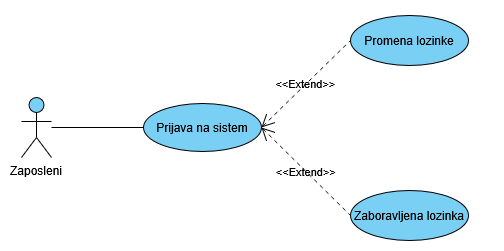
\includegraphics[width=\textwidth]{./dijagrami/dijagrami_slucajeva_upotrebe/slucaj_upotrebe_prijava_na_sistem.png} 
	\caption{Dijagram slučaja upotrebe ,,Prijava na sistem''}
\end{figure}

\begin{figure}[H]
	\centering
	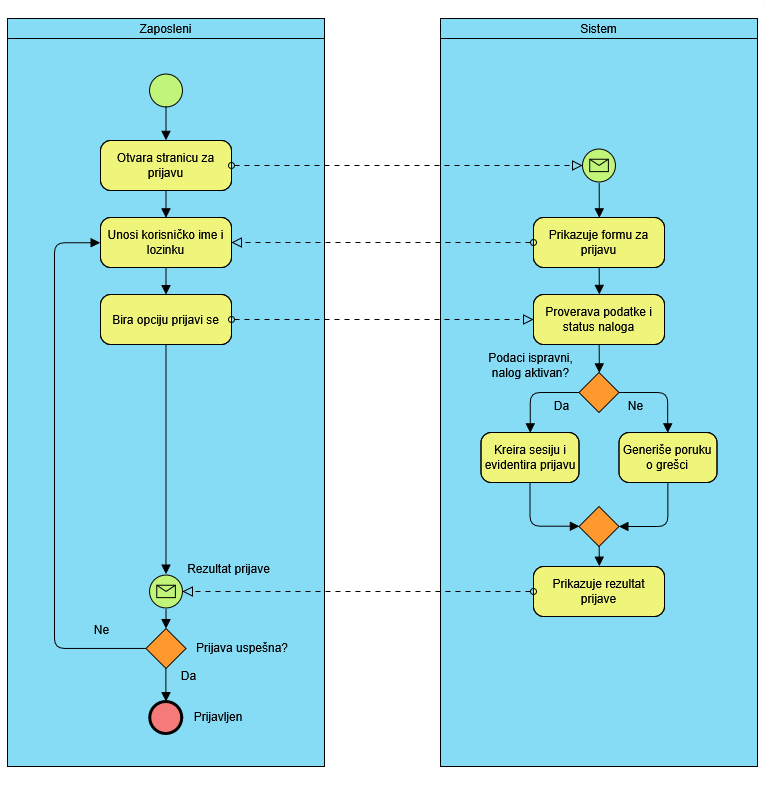
\includegraphics[width=\textwidth]{./dijagrami/bpmn/prijava_na_sistem.png} 
	\caption{BPMN dijagram saradnje ,,Prijava na sistem''}
\end{figure}

\newpage
